\documentclass[25pt, a0paper, portrait, leqno, margin=0mm, innermargin=25mm,
blockverticalspace=15mm, colspace=15mm, subcolspace=8mm]{tikzposter}

\usepackage{JRRG-tikzposter}
\usepackage{amsmath, amssymb}
\usepackage{poster-ehf2016}
\usepackage{theorem}
\usepackage{ehf2016} % http://xixon.epv.uniovi.es/ehf2016
\renewcommand{\baselinestretch}{1.05}
% \setlength{\parindent}{4em}

\setlength{\columnsep}{1.66em} % This is the default columnsep for all pages

\title{Stable Discontinuous Galerkin Approximations {\Large of the}
  Hydrostatic Stokes {\Large Equations}}
\author{F. Guillén González$^\dagger$, M.V. Redondo Neble$^\star$,
  J.R. Rodríguez Galván$^\star$}
\institute{\large $^\dagger$Departamento EDAN and IMUS,
  Univ. Sevilla. $^\star$Departamnto de Matemáticas, Univ. Cádiz.}

% ======================================================================%
\begin{document}
% ======================================================================%

\maketitle

\block{Anisotropic (Hydrostatic) Stokes Equations in Oceanography}{%
  % ======================================================================%
  \begin{multicols*}{3}
    \setlength{\parskip}{0.33\baselineskip}
    \textbf{Anisotropic Stokes (in particular, Hydrostatic) equations} are
    the centerpiece for more complex models in Oceanography in large
    scale domains, where
    $$
    \eps = \frac{\text{vertical scale}}{\text{horizontal scale}}
    \ \text{is very small}:
    $$

    \begin{equation}
      \tag{HydStokes}
      \left\{\;
        \begin{aligned}
          \dt\uu - \nu\Delta\uu + \gradx\pp &= \ff, \quad \text{in } \Omega,
          \\
          \eps^2\big\{\dt\vv - \Delta\vv \big\} + \partial_z\pp &= g, \quad \text{in } \Omega,
          \\
          \divx\uu +  \partial_z\vv &= 0, \quad \text{in } \Omega.
        \end{aligned}
      \right.
      \label{eq:hydstokes}
    \end{equation}

    In particular, the limit case, $ \eps=0 $ (the hydrostatic case)
    gives rise to the well known \textit{Primitive Equations of the
      ocean}.
    Their approximation has been studied by the authors
    in~\cite{Guillen-Redondo:16,Guillen-RRGalvan:hydrostatic:NUMAT:15,Guillen-RRGalvan:stabilized:SINUM:15,Guillen-RRGalvan:stokes:APNUM:16}.
    In the three later ones, two underlying \textbf{inf-sup constraints}
    for~(\ref{eq:hydstokes}) were shown:

    \begin{enumerate}
    \item A \textbf{LBB-like inf-sup} constraint.
    \item A new \textbf{Hydrostatic inf-sup} constraint, related to the
      vertical anisotropy of~(\ref{eq:hydstokes}):
      \begin{equation}
        \tag*{\ensuremath{(IS)^\VV}}
        \sup_{0\neq \pp \in \PP}
        \frac{\int_\Omega \pp \partial_z \vv}{\|\pp\|_{L^2(\Omega)}}
        \ge \ConstISv \|\partial_z\vv\|_{L^2(\Omega)},
        \
        \forall\, \vv\in H^1_z(\Omega).
        \label{eq:ISv}
      \end{equation}
    \end{enumerate}

    In order to \textbf{avoid these constraints}, making possible the use of
    standard finite elements for~(\ref{eq:hydstokes}), different
    techniques are proposed
    in~\cite{Guillen-RRGalvan:hydrostatic:NUMAT:15,Guillen-RRGalvan:stabilized:SINUM:15,Guillen-RRGalvan:stokes:APNUM:16}.

    \textbf{Here we show a different technique}, based in DG methods
    which verify the above inf-sup restrictions.
  \end{multicols*}
}

\block{Discontinous Galerkin Approximation}{%
  % ======================================================================%
  \begin{multicols*}{3}
    \setlength{\parskip}{0.33\baselineskip}
    We consider Interior Penalty
    (IP) methods that, for second order elliptic equations, were
    introduced by \cite{arnold_interior_1982} and for the isotropic
    Stokes equations (i.e.~for $\varepsilon=1$) have been recently
    studied by different authors (see e.g.~\cite{di_pietro_ern_2012}
    and references therein).

    Specifically, we \textbf{consider $P_k(\Th)$ discontinuous spaces
    $\Uh$, $\Vh$ and $\Ph$}, for approximation of
    % the broken (discontinous) polynomial space %
    % $P_k(\Th)$
    % $$
    % \Vh:=P_k(\Th) = \left\{
    %   v\in L^2(\Omega) \ | \ v\in \mathbb{P}_{k}(K), \ \forall K\in\Th \right\}
    % $$
    % and introduce the same discontinuous spaces for the velocity
    the velocity field $\wh=(\uh,v_h)\in\Uh\times\Vh$ and the pressure
    $\ph\in\Ph$.

    \section{\color{colorTwo}Anisotropic Bilinear Form and Norm\dotfill}

    The key for the well posedness of the discrete problem is in the
    introduction of the \textbf{anisotropic bilinear form} (depending
    on a penalty parameter $\mu>0$):
    $$
    a_h(\wh,\bwh) = \nu\sum_{i=1}^{d-1} a^{\text{sip}, \mu}(u_{h,i},\overline
    u_{h,i}) + \varepsilon^2 \,a^{\text{sip}, \mu/\varepsilon^2}(\vv,\bvh),
    $$
    where $a^{\text{sip}, \mu}$ is the well-known symmetric IP
    bilinear form,
    \begin{align*}
      a^{\text{sip},\mu}(\vv,\bv) &= \int_\Omega \gradh\vv\cdot\gradh\bv
      - \sum_{e\in\Eh} \int_e\Big( \average{\gradh\vv}\cdot n_e \jump{\bv}
        \\
      &+ \jump{\vv} \average{\gradh\bv}\cdot n_e \Big)
      + \mu\sum_{e\in\Eh} \frac{1}{h_e} \int_e \jump{\vv}\jump{\bv}.
    \end{align*}
    Here, $ \nabla_h$ denotes the broken (defined in elements)
    divergence operator, $\jump{\cdot}$ and $\average{\cdot}$ are the
    jump and average operators on the edges (or faces), denoted
    $e\in\Eh$.

    We must also consider the \textbf{anisotropic norm} for velocity
    $$
    \|\wh\|_\mathrm{vel} = \left(\|\uh\|_{\text{sip}}^2 +
      \|\partial_{z,h}\vh\|_{L^2(\Omega)}^2 + |\vh|_J^2\right)^{1/2},
    $$
    where $\|\cdot\|_{\text{sip}}$ is the norm associated to
    $a^{\text{sip},\mu}(\cdot,\cdot)$, $\partial_{z,h}$ is the broken
    partial derivative and $|\cdot|_J$ is the jump seminorm:
    $$
    \seminormJ{\vv} = \Big (\sum_{e\in\Eh} h_e^{-1} \norm[L^2(e)]{\jump\vv}^2 \Big ) ^{1/2}.
    $$

    \begin{lemma}[Partial coercivity for $a_h(\cdot,\cdot)$]
      \label{lemma:a_h-partial-coercivity}
      There exist $\overline{\mu} $ and $ \alpha >0$  (independent of $h$ and  $\varepsilon$), such that
      $ \forall \mu > \overline{\mu}$,
      $$
        a_h ( \wh, \wh ) \ge \alpha \Big ( \normsip{\uh}^2
        % + \sum_{i=1}^{d -1} ( \| \grad _h u _i \| _{L^2} ^2
        % + \seminormJ{u_i}^2 )
        + \seminormJ{\vh}^2  \Big ).
        $$
    \end{lemma}

    \begin{paragraph}{\textsc{Remark}}
      Lemma~\ref{lemma:a_h-partial-coercivity} does not provide
      control for $\|\partial_{z,h} \vh\|_{L^2(\Omega)}$ (and then for
      $\|\cdot\|_\mathrm{vel}$). It shall be recovered in
      Theorem~\ref{thm:discrete-inf-sup-stability}.
    \end{paragraph}

    \section{\color{colorTwo}Velocity-Pressure  Coupling\dotfill}

    Consider the standard IP velocity-pressure bilinear form,
    $$
    b_h(\wh, \ph )= -\int_{\Omega} \ph\, \gradh \cdot \wh +
    \sum_{e\in\Eh} \int_e \jump{\wh} \cdot n_e\, \average{\ph}
    $$
    and pressure seminorm, defined in
    $ H^1(\Th ) \supset P_{k}( \Th )$:
    $$
    |p|_P  = \Big ( \sum_{e\in\Ehi} h_e \, \| \jump{p} \|_{L^2(e)}^2 \Big )^{1/2}.
    $$

    \begin{lemma}[Stability for $b_h$] There exists
      \label{lemma:b_h-stability}
      $\beta > 0$ independent of $h$, such that
      $$
      \beta \, \| \ph \|_{L^2(\Omega)} \le \sup_{\wh \in \Wh \setminus
        \{0\}} \frac{b_h ( \wh, \ph )}{\normvel{\wh}}
      + |\ph|_P , \quad \forall \ph \in \Ph.
      $$
    \end{lemma}

    \section{\color{colorTwo}Discrete Problem and Well-Posedness \dotfill}

    We consider the discrete formulation for~(\ref{eq:hydstokes}):
    find $(\wh, \ph) \in \Wh \times \Ph$ such that, $\forall \bwh\in\Wh,\ \bph\in\Ph$,
    \begin{equation}
      \tag{P}
      \label{disc-var-pb}
      \left \{
        \begin{array}{l}
          a_h ( \wh, \bwh) +b_h ( \bwh, \ph ) = \int_{\Omega} f \, \bwh + \int_{\Gamma_s} \gs \, \bwh,
          \\
          \noalign{\smallskip}
          -b_h (\wh, \bph) + s_h (\ph, \bph)=0,
        \end{array} \right.
    \end{equation}
    where
    $s_h (\qh, r_h)= \displaystyle \sum_{e\in\Ehi} h_e \, \int_e
    \jump{\qh} \, \jump{r_h}$.

    Let $c((\wh,\ph),(\bwh,\bph))$ be the corresponding mixed bilinear
    form and let
    $$ \| (\wh, \ph)\|_{\Xh} = \Big ( \normvel{{\bf w}_h}^2 + \| \ph \|_{L^2}^2 +
    |\ph|_p^2\Big ) ^{1/2}.
    $$
    The following result implies well posedness of former
    discrete problem:
    % The following result holds for the corresponding mixed bilinear
    % form, $c((\wh,\ph),(\bwh,\bph))$:
    % depending $a_h(\cdot,\cdot)$
    % defined above, and on standard \textit{IP velocity-pressure},
    % $b_h(\wh,\ph)$ and \textit{jump} $s_h(\ph,\bph)$ bilinear
    % forms
    \begin{theorem}[Discrete inf-sup stability]
      \label{thm:discrete-inf-sup-stability}
      Assume that the
      penalty parameter $\mu$ in $a_h(\cdot,\cdot)$ is such that
      $ \mu > \overline{\mu}$. Then, there exists $\gamma >0$
      independent of $h$ and $\varepsilon$ such that, for all
      $(\wh, \ph) \in \Xh= \Uh\times\Vh\times\Ph$, one has
      $$
      \gamma \,\| (\wh, \ph)\|_{\Xh}\le \sup_{(\bwh,\bph)\in \Xh
        \setminus \{0\}} \frac{c_h ( (\wh, \ph), (\bwh,\bph) )}
      {\|(\bwh,\bph)\|_{\Xh} }.
      $$
    \end{theorem}
    \paragraph{\textsc{Proof}}(idea):
    \begin{enumerate}
    \item Lemma~\ref{lemma:a_h-partial-coercivity} provides control of
      $\normsip{\uh}^2$ and $\seminormJ{\vh}^2$.
    \item Lemma~\ref{lemma:b_h-stability} provides control of
      $\|p_h\|_{L^2(\Omega)}$.
    \item Discrete inf-sup condition~\ref{eq:ISv} is verified for
      $P_k$ elements, hence one has control of
      $\|\partial_{z,h} \vh\|_{L^2(\Omega)}$.
     \hfill$\blacksquare$
    \end{enumerate}
  \end{multicols*}
}

\block{Numerical Tests}{%
  \begin{multicols*}{4}
    \textbf{Cavity Test} for the discrete problem~(\ref{disc-var-pb}),
    programmed in \textbf{FreeFem++}~\cite{FreeFem++}, using the
    following data:
    \begin{itemize}
    \item Physical domain V/H ratio: $\eps=10^{-7}$.
    \item Viscosity: $\nu=1$.
    \item RHS functions: $\ff=0$, $g=0$.

    \item FE discretization:
      \begin{itemize}
      \item Admiensional domain $\Omega=[0,1]^2$, structured
        $32\times 32$ mesh ($h \sim 10^{-2}$).
      \item $P_1$ elements for velocity \& pressure.
      \end{itemize}
    \item Dirichlet boundary conditions (B.C.). Let
      $\Gamma_S=\mbox{surface boundary}$, we take:
      \begin{itemize}
      \item $u=x(x-1)$ on $\Gamma_S$,
      \item $u=0$ on $\partial\Omega \setminus \Gamma_S$,
      \item $v=0$ on $\partial\Omega$.
      \end{itemize}
    % \item pEpsilon  = 1.0e-10; // Penalty epsilon in p-equations
    \item B.C. are \textbf{imposed weakly}, using the Nitsche
    method.

  \item \textit{How to determinate adequate IP and B.C. (Nitsche)
      penalty parameters?}
    \begin{center}
      \textbf{\textit{Not easy!}}
    \end{center}
    We set:
    \begin{itemize}
    \item IP Penalty parameter\dotfill $\mu=10^{2}$,
    \item B.C. Penalty\dotfill $\eta = 10^{2}$.
    \end{itemize}
  \end{itemize}

    \begin{tabular}{@{}c@{}}
      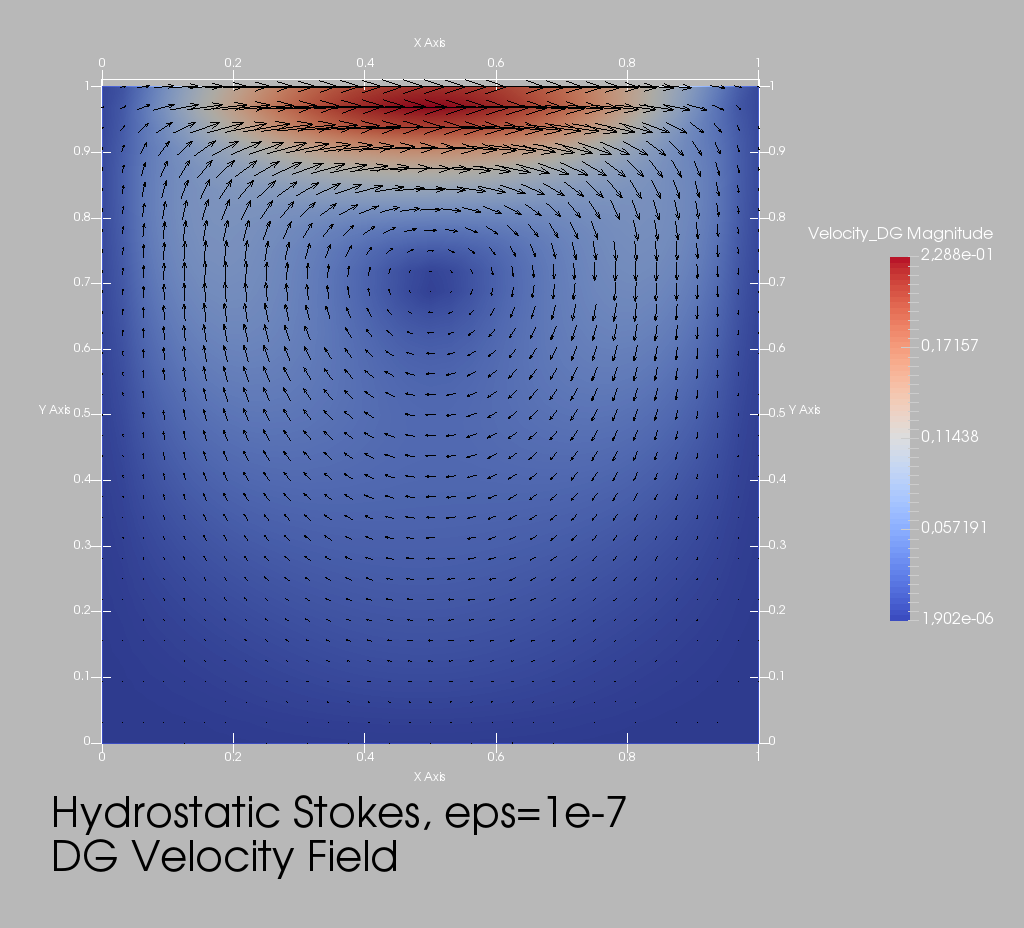
\includegraphics[width=1.0\linewidth]{hydstokes-DG-cavity-vel}
      \\
      Velocity field.
    \end{tabular}
    \begin{tabular}{@{}c@{}}
      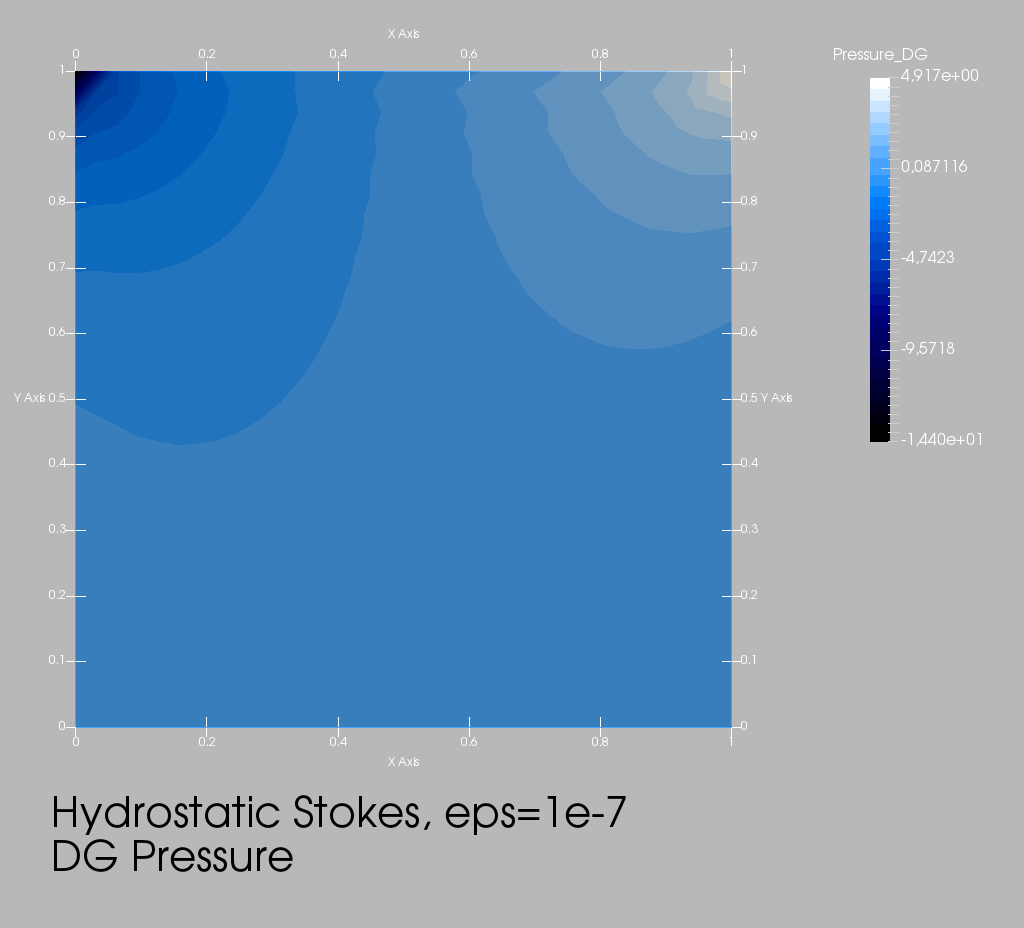
\includegraphics[width=1.0\linewidth]{hydstokes-DG-cavity-pres}
      \\
      Pressure iso-values.
    \end{tabular}
  \end{multicols*}
}

\block{}{%
  \begin{multicols*}{3}
    \footnotesize
    \section*{Acknowledgements} % If any
    The first author has been partially financed by MINECO grants
    MTM2015-69875-P (Spain) with the participation of FEDER. The second
    and third ones are also partially supported by the research group
    FQM-315 of Junta de Andalucía (Spain).
    \begin{thebibliography}{99}
      \footnotesize
    \bibitem{Guillen-Redondo:16}
      F.~Guillén-González and M.~V.~Redondo-Neble.
      \newblock Convergence and error estimates of a viscosity-splitting
      finite-element schemes for the primitive equations.
      \newblock Submitted.

    \bibitem{Guillen-RRGalvan:hydrostatic:NUMAT:15}
      F.~Guillén-González and J.~R. Rodríguez-Galván.
      \newblock Analysis of the hydrostatic {Stokes} problem and finite-element
      approximation in unstructured meshes.
      \newblock {\em Numerische Mathematik}, 130(2):225--256, June 2015.

    \bibitem{Guillen-RRGalvan:stabilized:SINUM:15}
      F.~Guillén~González and J.~R. Rodríguez~Galván.
      \newblock Stabilized {Schemes} for the {Hydrostatic} {Stokes} {Equations}.
      \newblock {\em SIAM Journal on Numerical Analysis}, 53(4), January 2015.

    \bibitem{Guillen-RRGalvan:stokes:APNUM:16}
      F.~Guillén-González and J.R. Rodríguez~Galván.
      \newblock On the stability of approximations for the {Stokes} problem using
      different finite element spaces for each component of the velocity.
      \newblock {\em Applied Numerical Mathematics}, 99:51--76, January 2016.

    \bibitem{arnold_interior_1982}
      Douglas~N. Arnold.
      \newblock An {Interior} {Penalty} {Finite} {Element} {Method} with
      {Discontinuous} {Elements}.
      \newblock {\em SIAM Journal on Numerical Analysis}, 19(4):742--760, August
      1982.

    \bibitem{di_pietro_ern_2012}
      D.~A.~Di~Pietro and A.~Ern.
      \newblock {\em Mathematical {Aspects} of {Discontinuous} {Galerkin} {Methods}}.
      \newblock Springer, Berlin; New York, 2012.

    \bibitem{FreeFem++}
      F.~Hecht.
      \newblock New development in freefem++.
      \newblock {\em J. Numer. Math.}, 20(3-4):251--265, 2012.
    \end{thebibliography}
  \end{multicols*}
}
\end{document}

%%% Local Variables:
%%% coding: utf-8
%%% mode: latex
%%% TeX-engine: xetex
%%% ispell-local-dictionary: "english"
%%% End:
